\documentclass{beamer}

\usepackage{amsmath,amsfonts,amssymb}
\usepackage{graphicx}
\usepackage{tikz}

\title{How to Conduct Interdisciplinary Research}
\subtitle{Strategies for Integrating Knowledge Across Fields}
\author{Morten Hjorth-Jensen}
\date{March 24, 2026, DScience workshop}

\begin{document}

\frame{\titlepage}

%------------------------------------------------

\begin{frame}{Motivation}

Many of today's scientific challenges cannot be solved
within a single discipline.

Examples include

\begin{itemize}
\item climate modeling
\item artificial intelligence and neuroscience
\item quantum computing and materials science
\item computational biology
\item financial engineering 
\end{itemize}

These problems require integrating knowledge
from multiple scientific fields.

\end{frame}


\begin{frame}{Scientific discovery}

Computational Science and Data Science have transformed scientific discovery.

Historically progress relied on

\begin{itemize}
\item improved algorithms
\item increased computational power
\item large-scale simulations
\end{itemize}

Examples include

\begin{itemize}
\item climate modeling
\item lattice quantum field theory
\item materials discovery
\item Neurotechnology and many other
\end{itemize}

However, many emerging scientific challenges involve
\textbf{multi-scale and highly complex systems} that
cannot be solved by computational power alone.

\end{frame}


\begin{frame}{Three Pillars of Future Discovery}
\centerline{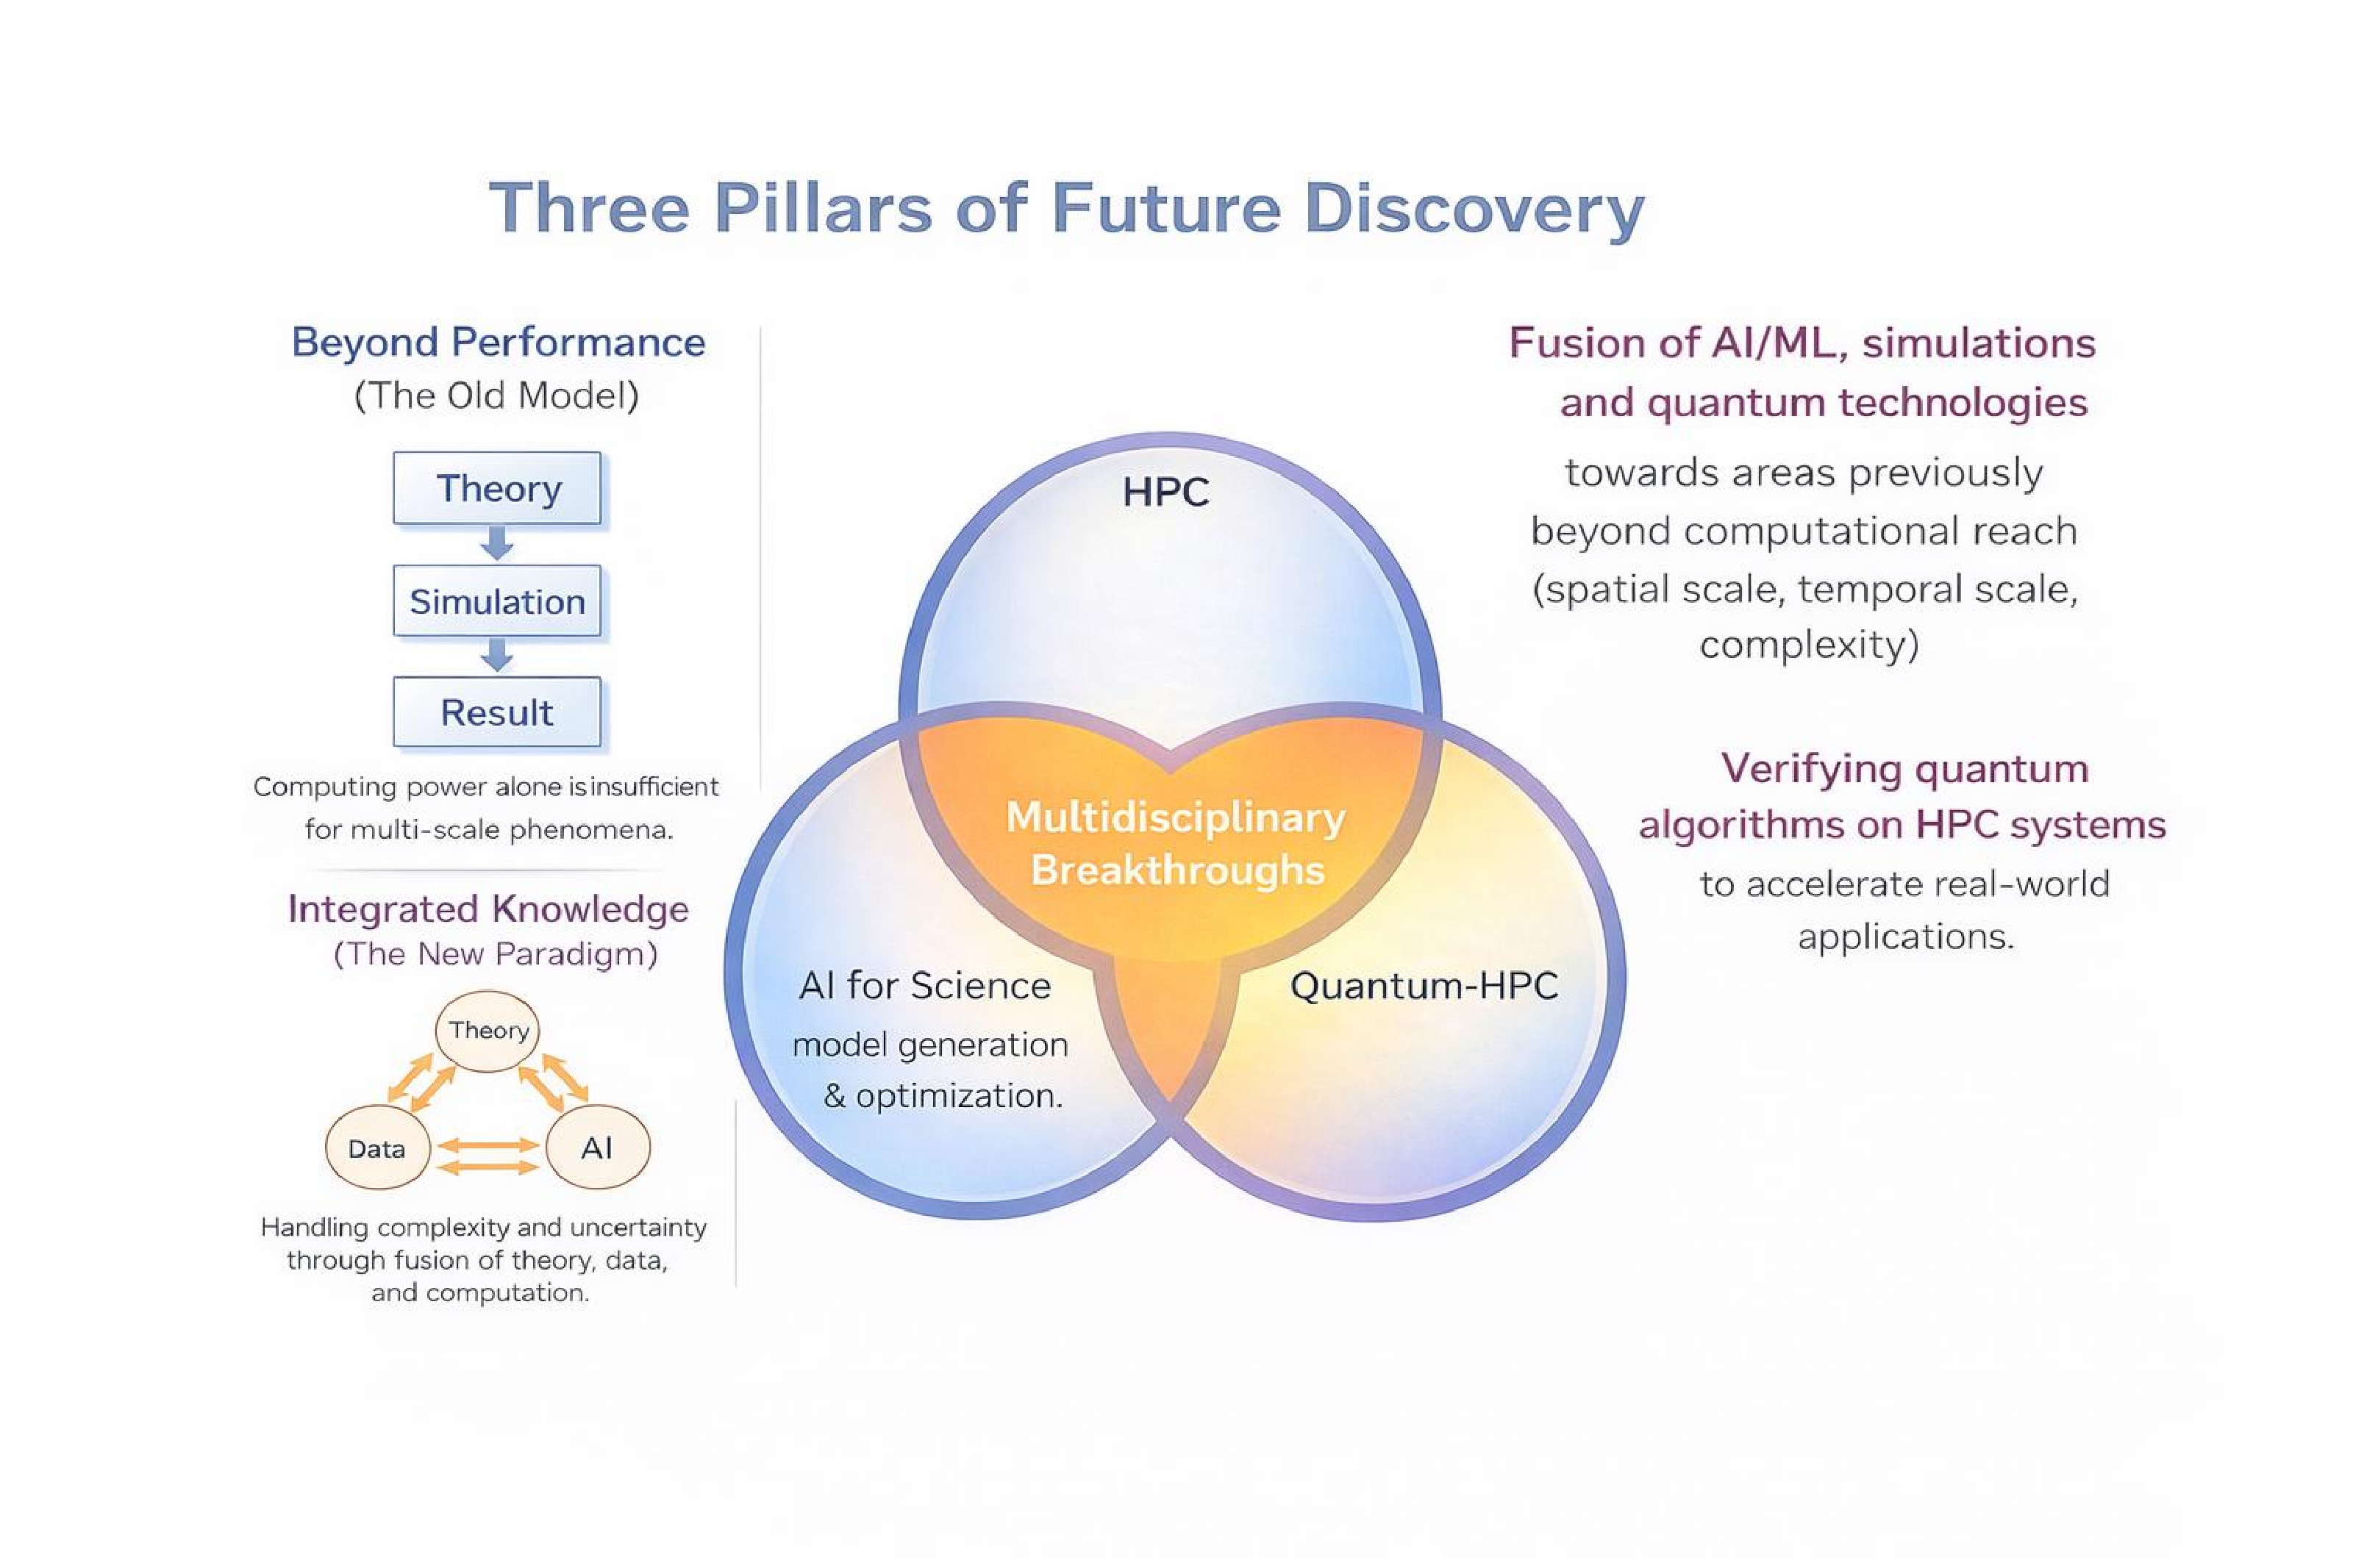
\includegraphics[width=1.0\linewidth]{Futurevision.pdf}}
\end{frame}



\begin{frame}{Three Pillars of Future Discovery}

Future advances in computational science will rely on
a fusion of three core pillars:

\begin{center}

Theory \\
Simulation / HPC \\
AI/ML and Quantum Technologies

\end{center}

These elements form an integrated ecosystem where

\begin{itemize}
\item theory guides modeling
\item simulations generate data
\item AI extracts patterns
\item quantum technologies extend computational capabilities
\end{itemize}

\end{frame}



%------------------------------------------------

\begin{frame}{The Limits of the Old Paradigm}

Traditional scientific computing relied primarily on

\begin{itemize}
\item numerical algorithms
\item high-performance computing
\end{itemize}

While extremely successful, this approach faces limits:

\begin{itemize}
\item exponential complexity of many-body systems
\item multi-scale physical phenomena
\item large uncertainty in complex models
\item difficulty extracting insight from massive datasets
\end{itemize}

The future requires a new paradigm integrating
\textbf{theory, data, and computation}.

\end{frame}

%------------------------------------------------

\begin{frame}{The New Paradigm}

The emerging paradigm of computational science includes:

\begin{itemize}
\item AI-driven model discovery via LLMs, reinforcement learning, transformers and much more
\item hybrid simulation frameworks
\item quantum computing for specific algorithms, see for example \url{https://arxiv.org/abs/2603.08883}
\item integrated theory–data workflows
\end{itemize}

Key idea:

\begin{center}
\textbf{Fusion of science-based models and data-driven learning}
\end{center}

This enables exploration of systems that were previously
beyond computational reach. And will require interdisciplinary collaborations.

\end{frame}



%------------------------------------------------

\begin{frame}{What is Interdisciplinary Research?}

Interdisciplinary research involves

\begin{itemize}
\item integrating knowledge from different disciplines
\item combining methodologies
\item creating shared conceptual frameworks
\end{itemize}

Important distinctions:

\begin{itemize}
\item \textbf{Multidisciplinary}: disciplines coexist
\item \textbf{Interdisciplinary}: disciplines interact
\item \textbf{Transdisciplinary}: new frameworks emerge
\end{itemize}

\end{frame}

%------------------------------------------------

\begin{frame}{Why Interdisciplinary Research Matters}

Benefits include

\begin{itemize}
\item solving complex scientific problems
\item generating innovative research directions
\item connecting theory, experiment, and computation
\item enabling technological innovation
\end{itemize}

Many breakthroughs occur at the intersection of fields.

\end{frame}

%------------------------------------------------

\begin{frame}{Example: Physics and Machine Learning}

Recent examples include

\begin{itemize}
\item neural-network quantum states
\item machine learning for phase transitions
\item physics-informed neural networks
\item AI-driven discovery of materials
\end{itemize}

These developments illustrate how methods from
computer science can accelerate physics research.

\end{frame}

%------------------------------------------------

\begin{frame}{Example: Physics and Neuroscience}

Statistical physics has influenced neuroscience.

Examples include

\begin{itemize}
\item Hopfield networks and spin models
\item neural population dynamics
\item collective behavior in neural systems
\item connectome network analysis
\end{itemize}

This interaction has helped build theoretical
frameworks for understanding brain function.

\end{frame}

%------------------------------------------------

\begin{frame}{Example: Quantum Technology and AI}

Another emerging intersection is

\begin{itemize}
\item reinforcement learning for quantum control
\item machine learning for quantum error correction
\item quantum machine learning algorithms
\item hybrid quantum–classical optimization
\end{itemize}

These areas illustrate how interdisciplinary research
creates entirely new fields.

\end{frame}

\begin{frame}{Example: Large-Scale Brain Simulations}

Modern neurotechnology increasingly relies on large-scale simulations.

Examples include

\begin{itemize}
\item whole-brain network models
\item cortical microcircuit simulations
\item neural field equations
\item spiking neural networks
\end{itemize}

These simulations require

\begin{itemize}
\item high-performance computing
\item efficient numerical methods
\item large experimental datasets
\end{itemize}

Computational science methods play a central role in
developing scalable algorithms for these systems.

\end{frame}




\begin{frame}{Example: Fiancial engineering, AI nd Quantum}


\begin{itemize}
\item Financial markets feature high-dimensional, stochastic data, making them well-suited for both machine learning and quantum computing approaches  
\item Quantum optimization methods (e.g., QAOA, quantum annealing) offer new ways to tackle complex portfolio optimization problems with constraints  
\item Quantum-enhanced machine learning, such as quantum kernels, may better capture correlations in financial time series  
\item Quantum generative models (e.g., variational circuits, quantum Boltzmann machines) can help simulate financial distributions for risk analysis and scenario generation  
\end{itemize}

\end{frame}


\begin{frame}{Interdisciplinary Collaboration Network}

\begin{center}

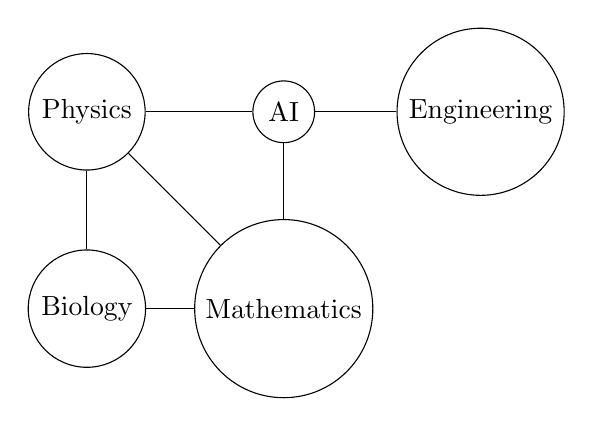
\begin{tikzpicture}[node distance=2.5cm]

\node (physics) [draw, circle] {Physics};
\node (ai) [draw, circle, right of=physics] {AI};
\node (bio) [draw, circle, below of=physics] {Biology};
\node (math) [draw, circle, below of=ai] {Mathematics};
\node (eng) [draw, circle, right of=ai] {Engineering};

\draw[-] (physics) -- (ai);
\draw[-] (physics) -- (bio);
\draw[-] (ai) -- (math);
\draw[-] (math) -- (bio);
\draw[-] (ai) -- (eng);
\draw[-] (physics) -- (math);

\end{tikzpicture}

\end{center}

Scientific breakthroughs often occur at the
intersections of these fields.

\end{frame}

%------------------------------------------------

\begin{frame}{Challenges in Interdisciplinary Research}

Common challenges include

\begin{itemize}
\item different scientific languages
\item different methodological traditions
\item communication barriers
\item differences in publication culture
\end{itemize}

These challenges require deliberate effort
to overcome.

\end{frame}

%------------------------------------------------

\begin{frame}{Building an Interdisciplinary Project}

Successful projects typically include

\begin{itemize}
\item a clearly defined scientific problem
\item complementary expertise
\item shared conceptual framework
\item collaborative infrastructure
\end{itemize}

The scientific problem should drive the collaboration.

\end{frame}

%------------------------------------------------

\begin{frame}{Developing a Shared Language}

Strategies include

\begin{itemize}
\item defining common terminology
\item identifying conceptual overlaps
\item documenting assumptions
\item encouraging cross-disciplinary learning
\end{itemize}

Communication is essential for successful collaboration.

\end{frame}

%------------------------------------------------

\begin{frame}{Designing Interdisciplinary Projects}

Key elements include

\begin{itemize}
\item defining clear research questions
\item combining complementary methodologies
\item establishing milestones
\item creating shared software and data resources
\end{itemize}

Good project management is crucial.

\end{frame}

%------------------------------------------------

\begin{frame}{Advice for PhD Students}

When you  enter interdisciplinary research projects, you should

\begin{itemize}
\item build strong foundations in one field
\item develop literacy in neighboring disciplines
\item cultivate curiosity and openness
\item collaborate with diverse research groups
\end{itemize}

Interdisciplinary expertise develops gradually.

\end{frame}

%------------------------------------------------

\begin{frame}{Developing Interdisciplinary Skills}

Important skills include

\begin{itemize}
\item communication across disciplines
\item computational literacy
\item data analysis skills
\item collaborative project management
\end{itemize}

These skills are increasingly valued in academia
and industry.

\end{frame}

%------------------------------------------------

\begin{frame}{Publishing Interdisciplinary Research}

Possible venues include

\begin{itemize}
\item interdisciplinary journals
\item computational science journals
\item domain-specific journals with cross-disciplinary focus
\end{itemize}

Selecting the right audience is important.

\end{frame}

%------------------------------------------------

\begin{frame}{Writing Interdisciplinary Grant Proposals}

Key elements include

\begin{itemize}
\item clear scientific question
\item justification of interdisciplinary approach
\item complementary expertise of team members
\item impact beyond a single field
\end{itemize}

Funding agencies increasingly encourage
cross-disciplinary collaborations.

\end{frame}

%------------------------------------------------

\begin{frame}{Interdisciplinary Research Centers}

Many universities now establish

\begin{itemize}
\item interdisciplinary research centers
\item cross-department institutes
\item collaborative graduate programs
\end{itemize}

These structures facilitate collaboration
between fields. DSscience is an example of this, same with the many new AI centers nationwide.

\end{frame}

%------------------------------------------------

\begin{frame}{Common Pitfalls}

Typical problems include

\begin{itemize}
\item superficial integration of disciplines
\item unclear research goals
\item lack of shared conceptual framework
\item poor communication
\end{itemize}

Successful interdisciplinary research requires
intentional planning.

\end{frame}

%------------------------------------------------

\begin{frame}{Best Practices}

Successful interdisciplinary researchers

\begin{itemize}
\item maintain depth in a core discipline
\item collaborate broadly
\item remain intellectually curious
\item cultivate communication skills
\end{itemize}

Interdisciplinary work combines intellectual
depth with collaborative breadth.

\end{frame}

%------------------------------------------------

\begin{frame}{Conclusion}

Interdisciplinary research is increasingly essential
for addressing complex scientific challenges.

Success depends on

\begin{itemize}
\item integrating knowledge across fields
\item strong collaboration
\item shared conceptual frameworks
\end{itemize}

The future of scientific discovery is most likely going to be
deeply interdisciplinary.

\end{frame}

\end{document}





## Quantum Machine learning for Finance



Quantum kernel methods encode classical data
into quantum states and evaluate similarity 
measures in
high‑dimensional Hilbert spaces. These approaches may offer new ways of
capturing complex 
correlations in financial time series.




## Applications to Neuroscience

Computational neuroscience represents another domain where the interplay
between AI and quantum 
technologies may prove valuable. The brain is a
highly complex dynamical system consisting of billions 
of interacting
neurons. Understanding neural computation requires tools capable of
analyzing massive 
datasets and modeling nonlinear dynamical
networks.

Machine learning already plays a central role in
neuroscience, particularly in analyzing neural 
recordings and building
models of neural activity. In the future, quantum machine learning
methods 
may offer alternative ways of representing high‑dimensional
neural data or modeling complex 
probability distributions arising in
neural activity patterns.

Another promising direction involves the use
of quantum simulation techniques to study models of 
neural dynamics.
Certain models of collective neural behavior exhibit similarities to
spin systems 
studied in statistical physics, suggesting that methods
developed for quantum many‑body physics may 
also provide new insights
into neural network dynamics.

# Future Strategies

Realizing the full potential of the interplay between artificial
intelligence and quantum technologies will require coordinated research
efforts across multiple disciplines.

First, interdisciplinary collaborations between physicists, computer
scientists, mathematicians, and engineers will be essential. Many of the
key challenges in this area lie at the intersection of these fields.

Second, education and training programs must evolve to reflect this
changing landscape. Future researchers will need expertise in physics,
numerical methods, machine learning, and quantum information science.

Third, large-scale research infrastructures that combine HPC resources,
experimental quantum platforms, and machine-learning-driven analysis
environments will play an increasingly important role.

# Conclusion

Artificial intelligence and quantum technologies are rapidly reshaping
the landscape of computational science. Their mutual interaction,
combined with advances in high-performance computing, is likely to
transform how scientific problems are approached and solved.

The integration of theory, simulation, machine learning, and quantum
hardware may enable entirely new forms of scientific discovery. As these
technologies continue to mature, their convergence will play a central
role in addressing some of the most challenging problems in physics,
chemistry, materials science, and beyond.

## References

1. I. Goodfellow, Y. Bengio, and A. Courville, *Deep Learning*, MIT Press
(2016).

2. J. Preskill, Quantum computing in the NISQ era, *Quantum* **2**, 79
(2018).

3. M. Bukov and F. Marquardt, Reinforcement learning for Quantum
Technology, *arXiv:2601.18953*, (2026).

4. F. Belliardo, F. Zoratti, F. Marquardt, and V. Giovannetti, Model-aware
reinforcement learning for high-performance Bayesian experimental design
in quantum metrology, *Quantum* **8**, 1555 (2024)

5. M. Schuld, and F. Petruccione, *Machine Learning with Quantum
Computers*, Springer-Verlag, Berling, 2021.
